\documentclass{article}[10pt]
\usepackage[utf8]{inputenc}
\usepackage{sectsty}
\allsectionsfont{\bfseries \sffamily}
\usepackage[linkcolor = red]{hyperref}
\usepackage{color}
\usepackage{setspace}
\usepackage{framed}
\usepackage{fancyhdr}
\usepackage{verbatim}
%\documentclass{amsart}
\usepackage{geometry}
\usepackage{alltt}
\usepackage{lastpage}
\usepackage{extramarks}
%\usepackage{mathabx}
\usepackage{parskip}
\usepackage{mathtools}
\usepackage{bbm}
\usepackage{amsfonts}
%\usepackage{titling}
\usepackage{cancel}
\usepackage{chngpage}
\usepackage{tikz}
\usepackage{soul}
\usepackage{array}
\usepackage{sectsty}
\usepackage{ascii}
\usepackage{xcolor}
%\usepackage{mdframed}
\allsectionsfont{\bfseries \sffamily}
%\usepackage{subfig}
%\usepackage{subfigure}
\usepackage{caption}
\usepackage{wrapfig}
\usepackage{subcaption}
\usepackage{enumerate}
\usepackage[usenames,dvipsnames]{color}
\usepackage{graphicx,float,wrapfig}
\usepackage{ifthen}
\usepackage{listings}
\usepackage{setspace}

\geometry{a4paper}

\linespread{2}

\def\changemargin#1#2{\list{}{\rightmargin#2\leftmargin#1}\item[]}
\let\endchangemargin=\endlist

\newcommand{\hmwkTitle}{Final Report}
\newcommand{\hmwkSubTitle}{}
\newcommand{\hmwkDueDate}{}
\newcommand{\hmwkClass}{GEOG 6000}
\newcommand{\hmwkClassTime}{}
\newcommand{\hmwkClassInstructor}{Professor Simon Brewer}
\newcommand{\hmwkAuthorName}{Evan Young}

%\pagestyle{fancy} 

% Margins
\topmargin=-0.5in      %
\evensidemargin=-.12in     %
\oddsidemargin=-.12in      %
%\marginparwidth = 0pt
\textwidth=6.5in        %
\textheight=9.25in       %
\headsep=0.25in         %

% Make title
\title{\vspace{2in}\textsf{\textmd{\textbf{{\Huge \hmwkClass:\ \hmwkTitle}\vspace{.2in}\hrule\vspace{.1in}\ifthenelse{\equal{\hmwkSubTitle}{}}{}{\\\hmwkSubTitle}}}\\\normalsize\vspace{0.1in}\\\vspace{0.1in}}\large{\textit{\hmwkClassInstructor\ \hmwkClassTime}}\vspace{3in}}
\date{}
\author{\textbf{\hmwkAuthorName}}

% Books 
% Applied Spatial Data Analysis in R -- Bivand
% Elements of Statistical Learning -- Hastie & Tibshirani
% Data Analysis and Statistics for Geography, Environmental Science, and Engineering -- Acevedo
% Generalized Additive Modelling -- Hastie & Tibshirani
% Google's PageRank and Beyond: The Science of Search Engine Rankings -- Langville
% Introduction to Stochastic Processes -- Lawler
% Pattern Recognition and Machine Learning -- Bishop

\begin{document}
\begin{titlegpage}
\maketitle
\thispagestyle{empty}
\end{titlepage}
\newpage
%
%
%\begin{center}
%\section*{Project Proposal}
%
%{\sffamily Name: } Evan Young
%
%{\sffamily Uid: } u0755450
%
%{\sffamily Email: }{\ttfamily evan.d.young@gmail.com}
%\\
%
%\end{center}
\begin{spacing}{1.5}
\colorbox[cmyk]{0.13, 0, 0, 0}{
%\begin{abstract} %\noindent
\parbox{\textwidth}{
\vspace{.05in}
\begin{abstract}%\noindent
\textit{In this paper we will look at the influence that ideological extremism held by a member of the United States House of Representatives has on the power and influence that they possess. In recent years we have seen broad coverage in the media of the virtual stand still in the volume of legislation coming out of Congress. Although control of the House has pass from liberal to conservative hands many times this congressional atrophy is quite unprecedented. Many have proposed that this disruption is due to the rise of the far-right Tea Party movement. While others have blamed the current Presidential administration�s uncooperative attitude. Through our analysis we will examine the datasets of bill cosponsorships made publicly available on GovTrack.us. This data will be used  to explore trends in ideological views and influence over the last 40 years. We will employ a linear model, a generalized additive model, and use categorical classification to examine these trends overtime. Geographical analysis will also used to observe how these trends manifest in different parts of the nation. }
\vspace{.1 in}
\end{abstract}}
}
\end{spacing}
\vspace{.2 in}
\section*{Introduction}
As we approach the end of another congress, we are quickly coming up on the close of the most unproductive congress in history. The 113th congress, at this time, is 180 bills behind the current record holder for the most unproductive congress, which happens to be the previous congress. This period of legislative drought is unprecedented and often attributed to an extremely polarized congress. Harry Enten, of the website FiveThirtyEight.com, has reported that Congress is the most divided it has been in almost one hundred years. This division begs the question, what is causing this division? There are many news outlets that quickly turn the blame on the rise of the Tea Party movement. However as you can see in Figure 1 it is possible that this is a downturn that began before the Tea Party movement's formation. 
\begin{figure}[H]
	\centering
	\begin{subfigure}[H]{.8\textwidth}
		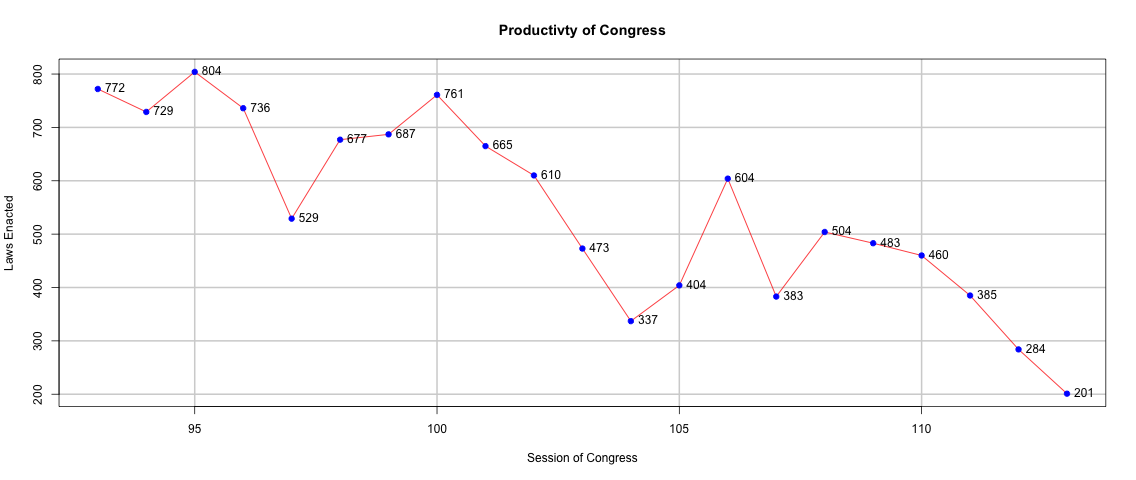
\includegraphics[width=\textwidth]{../prodCon.png}
		\caption*{Figure 1}
	\end{subfigure}
\end{figure}
On the other hand it could be that what would have been a temporary dip in productivity as been urged on by politically extreme members of the House of Representatives on both sides. It is clear from Figure 2 that there are strong trends towards the more extreme representative having more influence on both sides of the aisle. 
\begin{figure}[H]
	\centering
	\begin{subfigure}[H]{.4\textwidth}
		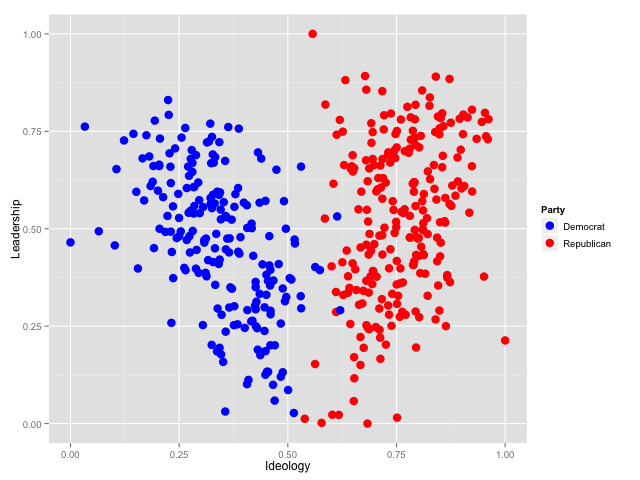
\includegraphics[width=\textwidth]{../charts/113chart.png}
		\caption*{Figure 2}
	\end{subfigure}
\end{figure}
Were we able to show that this circumstance is unique to the most recent sessions of Congress it would be reasonable to conclude that having ideologically extreme politicians in positions of great influence has contributed to the virtual halt in legislation. It is our hypothesis that this is the case. 
%\section*{Literature Review}
%To perform this analysis we will rely heavily on the academic works of a few authors. The 
\section*{Acquisition and Processing of the Data}
\subsection*{Source of the Data}
The Congressional cosponsorship data that we will be using is from Joshua Tauberer and his website {\color{blue}\href{http://govtrack.us}{GovTrack.us}}. In 2004, Tauberer founded GovTrack.us and used the cosponsorship data to establish leadership and ideological scores for each Senator and Representative of Congress from the 93rd Congress forward. The method of generating these metrics will be discussed at a further point in the paper. Tauberer has made the data on his website freely available with an open API and bulk downloading options. 

\newpage \quad
\newpage 
\section*{Statistical Methods}
\subsection*{Linear Model}
\newpage
\subsection*{Generalized Additive Model}
\newpage
\subsection*{Categorical Analysis}
\newpage
\section*{Conclusion}
\newpage
\section*{Literature Review}
\newpage
\section*{Bibliography}
\begin{figure}[p]
    \vspace*{-2cm} %\hspace*{-2cm}
    \makebox[1\linewidth]{
  		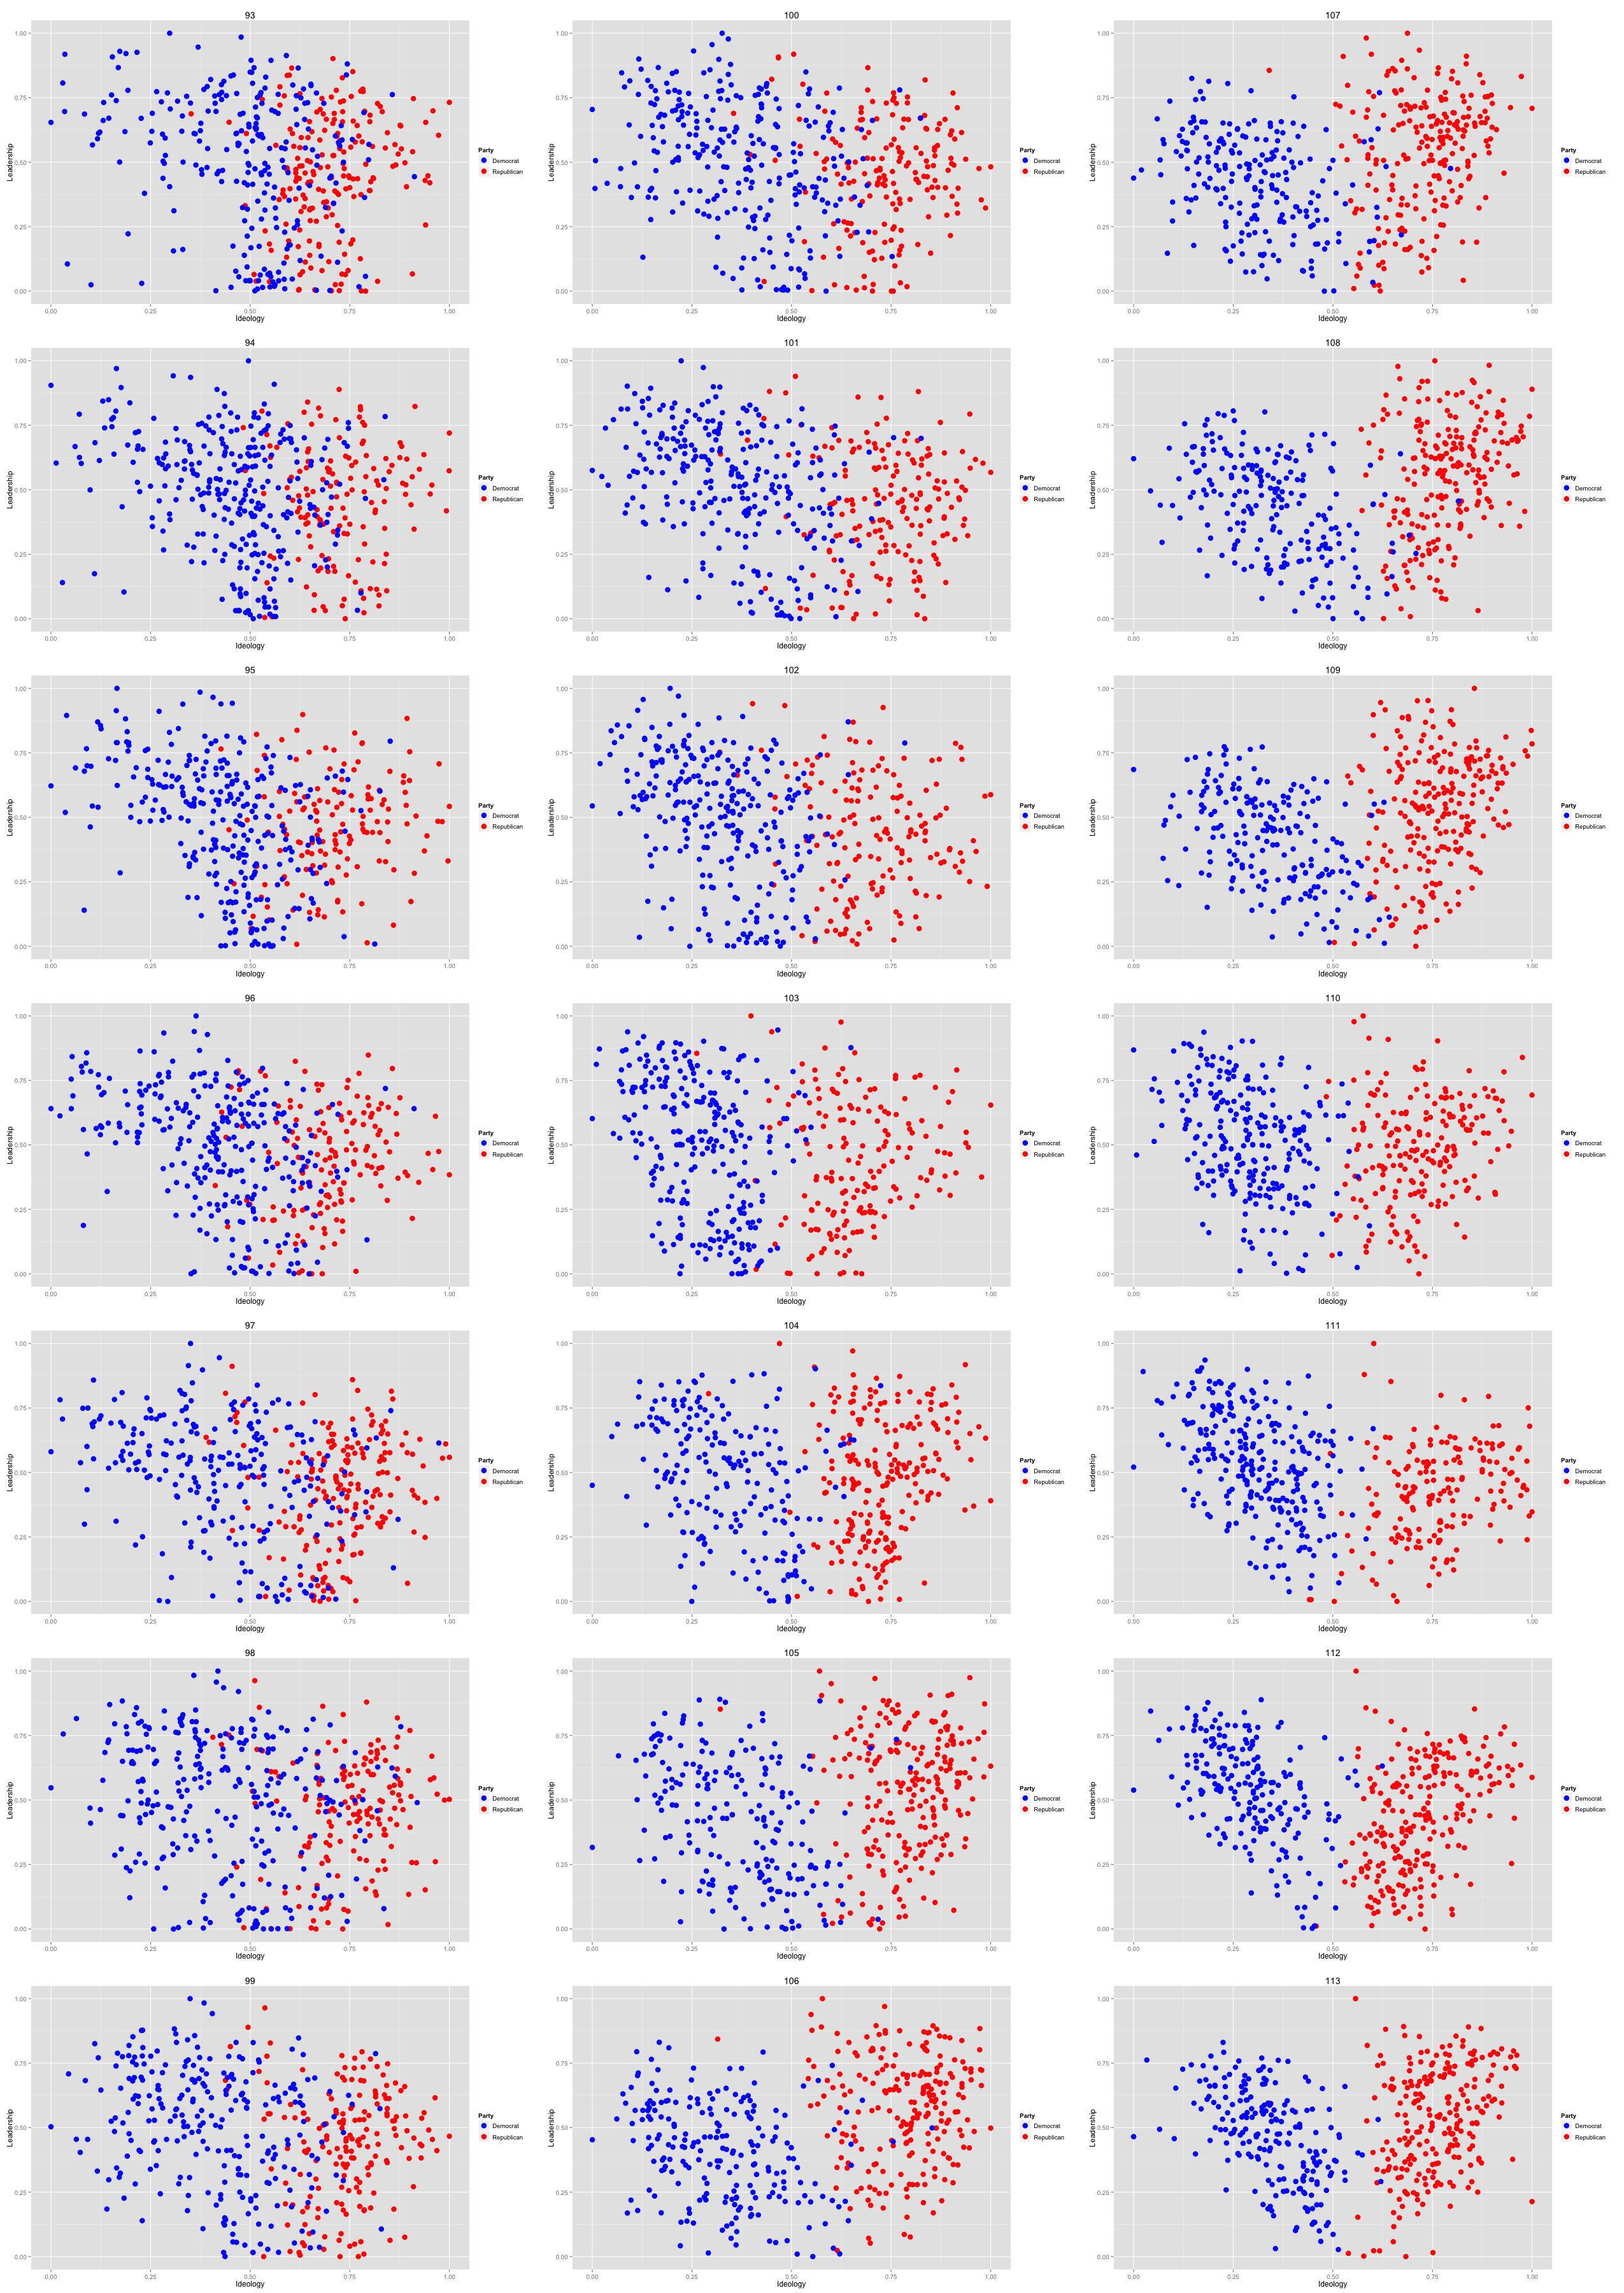
\includegraphics[width=1.2\linewidth]{../full.png}  	
    }
    \caption*{Figure 3 \\ Starts at top left and goes down each column}
\end{figure}
\end{document}
